\newpage
\section{Resultater (10 poeng)}\label{resultater-10-poeng}
\subsection{1. Multippel lineær regresjon}

\begin{table}[h!]
    \centering
    \begin{tabular}{lcccccc}
        \hline
        \textbf{Variabel} & \textbf{coef} & \textbf{std err} & \textbf{t} & \textbf{$p$-verdi} & \textbf{[0.025} & \textbf{0.975]} \\
        \hline
        \textbf{Intercept} & 47,4932 & 1,486 & 31.951 & 0,000 & 44,575 & 50,418 \\
        \textbf{Pclass}    & -6,4016 & 0,582 & -10,992 & 0,000 & -7,545 & -5,285 \\
        \textbf{FamilySize}     & -2.554 & 0,332 & -7,688 & 0,000 & -3.206 & -1.902 \\
        \textbf{Sex}     & -2.9129 & 1,034 & -2,818 & 0,005 & -4,943 & -0,883 \\
        \hline
    \end{tabular}
    \caption{Resultater fra multippel lineær regresjonsmodell for aldersestimering.}
    \label{tab:regresjon_alder}
\end{table}

Samlet utgjør modellen en determinasjonskoeffisient på $R^2 = 0.224$. Dette betyr at den forklarer 22.4\% av variansen i alderen til passasjerene. Forklaringsevnen til modellen er relativt lav, men kan skyldes at alder påvirkes av ytterlige faktorer utover det vi har vi har tatt for oss og datasettet har tilgjengelig.  Variablene er likevel statistisk signifikant, noe som viser at de har en reell sammenheng med alder.

Regresjonslikningen: 

$$\textit{Age} = 47.493 - 6.402*\textit{Pclass}-2.554*FamilySize-2.913*\textit{Sex}$$

\textbf{Forklaringsvariabler:} 

\textit{Age} (Intercept) \\
Den gjennomsnittlige alderen til en passasjer som er mann, har ingen familiemedlemmer om bord og ikke tilhører noen klasse er 47.49 år gammel. Ettersom at hver passasjer tilhører en klasse, så er den høyeste mulige predikerte alderen omtrent 41.1 år dersom passasjeren tilhører 1. klasse.
Vi ser også at modellen vi endte opp med, vil maksimalt estimere alder til å være 41.1 år ettersom alle forklaringsvariable har negativ korrelasjon. Dette medfører at alle eldre passasjerer i datasettet konsekvent vil estimeres til å ha lavere alder enn de faktisk har.

\textit{Pclass} \\ For hver lavere klasse en passasjer tilhører (eks. klasse 1. til klasse 2.), reduseres den forventede alderen i snitt med 6.38 år (($\beta_1 = -6.4016, p < 0.000$). 95\% konfidensiellintervallet $[-7.545, -5.285]$ viser god presisjon i estimatet og en tydelig effekt.

\textit{FamilySize} \\ For hvert ekstra familiemedlem en passasjer hadde ombord (søsken, forelder, barn, ektefelle), reduserer den forventede alderen i snitt med 2.55 år ($\beta_2 - 2.554, p < 0.000$). Konfidensintervallet ligger på 95\% ligger mellom [-3.206, -1.902], som også her viser god presisjon når vi estimerer familie størrelse. Dette kan henge sammen med at barn oftere reiste sammen med familie. Den skiller dog ikke mellom en passasjer som reiste med foreldre, og en annen som reiste med egne barn.

\textit{Sex} \\ Resultatet viser at kvinner i snitt er 2.91 år yngre enn det menn er ($\beta_3 = -2.913, p = 0.001$). Denne variabelen har det høyeste standardavviket på 1.04 og det bredeste konfidensintervallet $[-4.943, -0.883]$, noe som indikerer at aldersforskjellen mellom menn og kvinner har større usikkerhet og variasjon enn de andre utvalgte variablene.


%\textit{SibSp} ($\beta_2 = -3.91, p < 0.000$) står statistisk signifikant og viser at hvert søsken/ektefelle en passasjer hadde ombord, reduserte den forventede alderen med 3.91 år. \textit{Parch} ($\beta_3 = -0.95, p = 0.124$) er ikke statistisk signifikant med et 5\% signifikansnivå. Dette kan som nevnt i metodekapitellet, skyldes at variabelen inneholder foreldre som trekker alder opp og barn som trekker barn ned. Dette betyr at vi har tilstrekkelig med bevis for at antall foreldre eller barn en passasjer hadde om bord har en reell effekt på alderen. 

\noindent
\begin{minipage}[c]{0.48\textwidth}
    \textbf{Residualplott} \\
    Residualplottet har en liten antydning til vifteform. Spredningen i residualene øker med høyere estimerte alder. Dette betyr at variansen til feilleddene ikke er konstante. Modellen treffer gradvis mindre nøyaktig for  høyere alder, men at det ikke er mulig å estimere alder for eldre passasjerer. Figuren viser at den høyeste predikerte alderen modellen oppnådde var $\approx 41 år$, noe som skyldes at alle forklaringsvariablene har en negativ korrelasjon.

\end{minipage}
\hfill
\begin{minipage}[c]{0.48\textwidth}
    \centering
    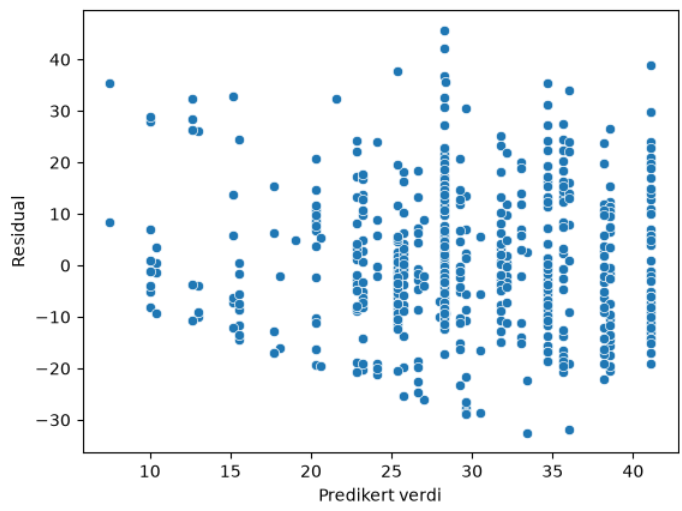
\includegraphics[width=0.89\linewidth]
    {Images/linear_scatterplot.png}
    \captionof{figure}{Residualer mot predikert alder}
    \label{fig:linear_scatterplot.png}
\end{minipage}

\noindent
\begin{minipage}[c]{0.48\textwidth}
    \textbf{QQplott} \\
        Punktene i figuren følger i stor grad linjen, noe som antyder at feileddene i hovedsak er tilnærmet normalfordelte.
        Punktene har noe positiv skjevhet i høyre hale, da enkeltene av punktene i den øvre delen legger seg litt ovenfor linjen. Skjevheten her skyldes at det modellen kun har forklaringsvariabler med negativ korrelasjon, noe som også medfører at eldre passasjer estimeres som mye yngre enn de egentlig er. 

\end{minipage}
\hfill
\begin{minipage}[c]{0.48\textwidth}
    \centering
    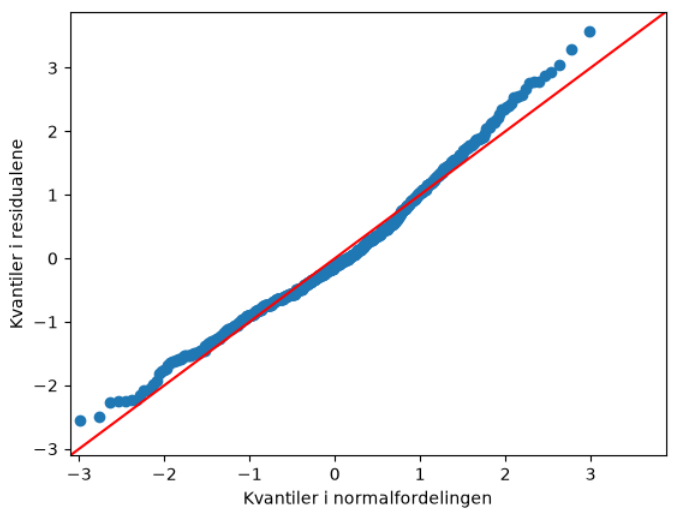
\includegraphics[width=0.89\linewidth]
    {Images/linear_qqplot.png}
    \captionof{figure}{Residualene fra aldersmodellen}
    \label{fig:linear_qqplot}
\end{minipage}

\subsection{2. Klassifisering}
Etter oppdeling av datasettet, består treningssettet av 534 rader, valideringsettet av 178 rader og testsettet av 179 rader. For modellen med imputering er rader som mangler alder har blitt estimert inn ved hjelp av OLS fra forrige del. For analysen uten imputering fjernes radene hvor alder mangler.

\begin{table}[htbp]
  \centering
  \begin{minipage}[c]{0.48\textwidth}
    \centering
    \caption{Valideringsresultater for KNN-modellene med imputering ved OLS.}
    \label{tab:knn_validering_1}
    \begin{tabular}{lcc}
      \hline
      \textbf{Modell} & \textbf{Beste \textit{k}} & \textbf{Feilrate} \\ \hline
      \textbf{Modell 1:} \textit{Sex} + \textit{Age} & 29 & 0.2078 \\ 
      \textbf{Modell 2:} + \textit{Pclass} & 11 & 0.1629 \\ 
      \textbf{Modell 3:} + \textit{FamilySize} & 19 & 0.1741 \\ \hline % Samme feilrate på denne og modell 2???
    \end{tabular}
  \end{minipage}
  \hfill
  \begin{minipage}[c]{0.48\textwidth}
    \centering
    \caption{Valideringsresultater for KNN-modellene uten imputering.}
    \label{tab:knn_validering_2}
    \begin{tabular}{lcc}
      \hline
      \textbf{Modell} & \textbf{Beste \textit{k}} & \textbf{Feilrate} \\ \hline
      \textbf{Modell 1:} \textit{Sex} + \textit{Age} & 29 & 0.2253 \\ 
      \textbf{Modell 2:} + \textit{Pclass} & 103 & 0.1901 \\ 
      \textbf{Modell 3:} + \textit{FamilySize} & 95 & 0.1830 \\ \hline
    \end{tabular}
  \end{minipage}
\end{table}

Baseline feilraten ligger på $\approx38\%$ med imputering og $\approx40$ uten imputering. Alle modellene får dermed en feilrate som er lavere enn baseline.

For modellene med imputering, oppnår modell 2 (\textit{Sex} + \textit{Age} + \textit{Pclass}) best resultat med en feilrate på $16.29\%$ og $k = 11$. Ved å fjerne klassen passasjerene tilhører (\textit{Pclass}) øker feilraten til $20.78\%$, og dersom familiestørrelsen (\textit{FamilySize}) inkluderes øker feilraten til $17.41\%$. Familiestørrelsen gir ingen forbedring ovenfor modell 2 ved imputering av alder.

\noindent
\begin{minipage}[c]{0.48\textwidth}
    \centering
    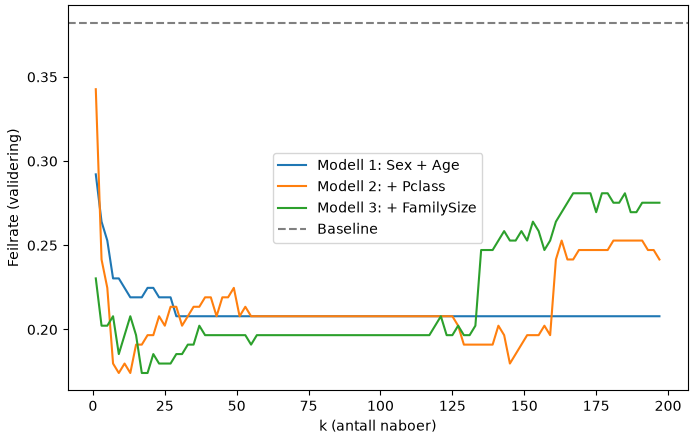
\includegraphics[width=1\linewidth]
    {Images/valideringssett_knn+ols.png}
    \captionof{figure}{Validering av modellene med imputering ved OLS}
    \label{fig:Valideringssett_ols}
\end{minipage}
\hfill
\begin{minipage}[c]{0.45\textwidth}
    \centering
    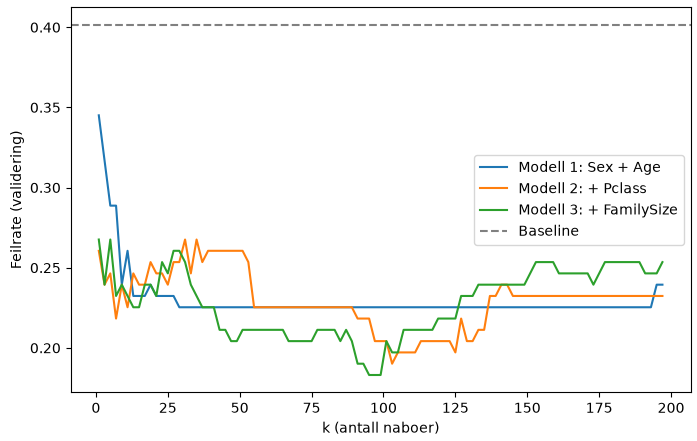
\includegraphics[width=1\linewidth]
    {Images/valideringssett_knn.png}
    \captionof{figure}{Validering av modellene uten imputering}
    \label{fig:Valideringssett}
\end{minipage}

For modellene hvor radene som mangler alder er fjernet gir modell 3 det beste resultatet, med en feilrate på $18.3\%$ og $k=95$. I motsetning til det andre resultatet, så ga familiestørrelsen en liten forbedring ovenfor modell 2.

Etter valg av modeller basert på resultatene fra validering evalueres de basert på testsettet. For modellen hvor imputering er brukt har modell 2 blitt benyttet, mens modell 3 har blitt benyttet for datasettet hvor radene som manglet alder er fjernet.

Med imputering fra multippel lineær regresjon:

$Nøyaktighet = \frac{TP+TN}{Observasjoner} = \frac{43+101}{179}\approx0.8045$

Rader hvor alder mangler er fjernet:

$Nøyaktighet = \frac{TP+TN}{Observasjoner} = \frac{42+72}{143}\approx0.7972$

Ved imputering av alder får modellen en nøyaktighet på $80.45\%$. Blant passasjerene som omkom, ble $91.8\%$ klassifisert riktig. 101 av 110 omkomne passasjerer ble korrekt klassifisert, mens de resterende 9 ble feilklassifisert som omkomne. Blant de overlevende ble $62.3\%$ klassifisert riktig, mens de resterende 23 ble feilklassifisert som overlevende.

Ved å kutte ut rader som mangler alder oppnår modellen en nøyaktighet på $79.72\%$. $88.9\%$ av passasjerene som omkom ble klassifisert riktig. Blant de som overlevde ble $67.7\%$ klassifisert riktig. Modellen hvor alder er kuttet ut er $\approx 5\%$ mer presis på klassifisering av overlevende og $\approx 3\%$ mindre presis på å klassifsering av omkomne.

\noindent
\begin{minipage}[c]{0.40\textwidth}
    \centering
    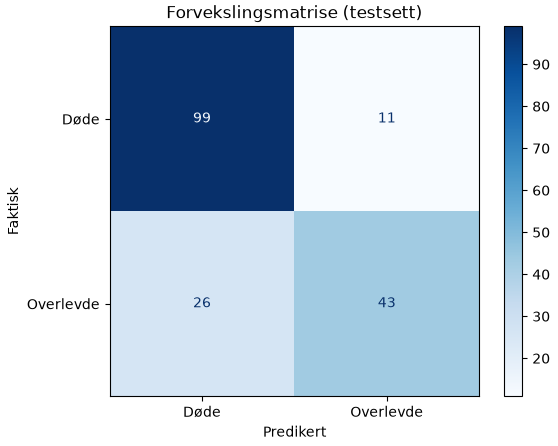
\includegraphics[width=1\linewidth]
    {Images/forvekslingsmatrise_knn+ols.png}
    \captionof{figure}{Testresultat med imputering ved OLS}
    \label{fig:Forvekslingsmatrise med imputering ved OLS}

\end{minipage}
\hfill
\begin{minipage}[c]{0.40\textwidth}
    \centering
    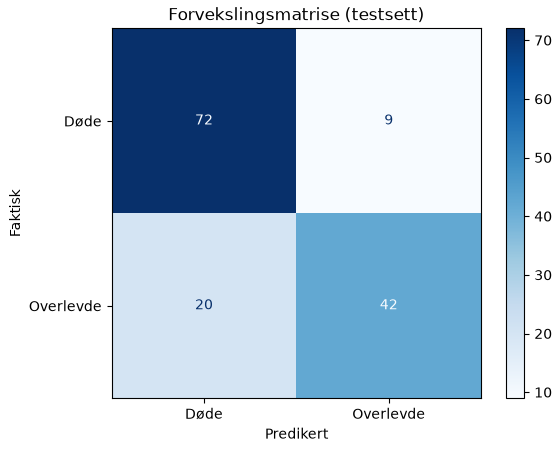
\includegraphics[width=1\linewidth]
    {Images/forvekslingsmatrise_knn.png}
    \captionof{figure}{Testresultat uten imputering}
    \label{fig:Forvekslingsmatise uten imputering ved OLS}
\end{minipage}